There are many ways to design and implement applications for a distributed cluster, a set of
computers, typically labeled as (computational) nodes, that have their own independent processors
and memory and are connected together with a computer network so that they can cooperate on solving
difficult problems. In the context of \gls{hpc}, such distributed clusters are called
\emph{supercomputers}, and one of their distinguishing features is that all the computers of the
cluster reside within one physical location, and they are connected with a very high-speed and
low-latency network. Even though there are other kinds of distributed clusters, such as data
centers or cloud-based systems, this thesis focuses exclusively on \gls{hpc} systems
and supercomputers; therefore, the term (distributed) cluster will denote an \gls{hpc}
cluster in the rest of the text.

Distributed applications are implemented using various \emph{programming models} that allow expressing
communication patterns which enable individual cluster nodes to cooperate and exchange data, and
thus efficiently utilize available computational resources. Communication between nodes is crucial,
as that is what allows distributed clusters to offer unparalleled performance by distributing the
computational load among multiple computers and thus achieving speedup through parallelization.

This thesis is focused on a particular subset of task-based programming models and their
interaction with \gls{hpc} clusters. The goal of this chapter is to specify this
subset. First, it provides a broad overview of the most popular approaches for implementing
distributed and parallel applications (with particular focus on \gls{hpc} use-cases),
and then it gradually concretizes which niches of this diverse area are most relevant to the topic
of this thesis.

\section{Parallel programming models}
This section describes the most important representatives of programming models that are used in
the world of supercomputing. It divides the programming models into two broad categories: models
that express parallelization and network communication explicitly, and models that do so
implicitly.

\subsection*{Explicit parallelization}
One way to design distributed applications is to leverage programming models that express the
parallelization of computation and the exchange of data between nodes explicitly. This has been the
predominant way of creating \gls{hpc} software for many years, and it is still very
popular today~\cite{mpiusagestudy1,mpiusagestudy2,mpiusagestudy3}. Below are a few examples of these explicit approaches.

\begin{description}[wide=0pt]
	\item[Message passing] has historically been the most popular method for implementing \gls{hpc} software. In
		this model, a distributed computation is performed by a set of processes with separate memory
		address spaces that are typically executed across multiple nodes. The processes cooperate together
		to solve complex problems by exchanging network messages (hence the term \emph{message passing}).
		Message passing applications are commonly implemented using the
		\gls{spmd}~\cite{spmd} programming model, where the implementation logic of
		all the processes participating in the computation is embedded within a single program.

		The most popular representative of this programming model is the
		\gls{mpi}~\cite{mpi} framework, which is used by a large number of
		existing \gls{hpc} applications~\cite{mpiusagestudy2}. It defines a set of
		communication primitives, operators and data types, which can be used to perform computations,
		exchange data and synchronize progress between either two (\emph{point-to-point communication}) or multiple
		(\emph{collective communication}) processes running on remote nodes. \Autoref{lst:mpi-example} shows a simple
		\gls{mpi} program designed to be executed in two (potentially distributed) processes.
		The first process sends a number to the second process, which waits until that number is received,
		and then prints it. Notice how network communication and process synchronization is expressed
		explicitly, by calling the \texttt{MPI\_Send} and \texttt{MPI\_Recv} functions. We can also
		see the \gls{spmd} paradigm in practice, because the code for both processes is
		interleaved within the same program.

		\begin{listing}[h]
			\begin{minted}[fontsize=\footnotesize]{c}
#include <mpi.h>
#include <stdio.h>

int main() {
	MPI_Init(NULL, NULL);

	// Find out the ID of this process
	int process_id;
	MPI_Comm_rank(MPI_COMM_WORLD, &process_id);

	if (process_id == 0) {
		// Send one integer to process 1
		int value = 42;
		MPI_Send(&value, 1, MPI_INT, 1, 0, MPI_COMM_WORLD);
	} else if (process_id == 1) {
		// Receive one integer from process 0
		int value = 0;
		MPI_Recv(&value, 1, MPI_INT, 0, 0, MPI_COMM_WORLD, MPI_STATUS_IGNORE);
		printf("Process 1 received number %d from process 0\n", value);
	}

	MPI_Finalize();

	return 0;
}
		  	\end{minted}
			\caption{\gls{mpi} program implemented in \texttt{C}}
			\label{lst:mpi-example}
		\end{listing}

	\item[\gls{pgas}~\cite{pgas}] is a relatively similar programming model, which also often employs the \gls{spmd}
		paradigm. Where it differs from message passing is in the way it expresses communication between
		processes. Message passing processes share their memory by communicating with other processes,
		while PGAS provides an abstraction of a shared memory address space and allows processes to
		communicate through it\footnote{To paraphrase the famous ``Do not communicate by sharing memory; instead, share memory by communicating'' quote that originates from the \texttt{Go} programming
		language community.}. \gls{pgas} provides an illusion of a
		global memory address space that is available to processes that participate in the communication,
		which makes it slightly less explicit in terms of expressing the communication patterns within the
		program, because it translates certain memory operations into network messages on behalf of the
		programmer.

		\gls{pgas} programs also often employ \emph{one-sided communication} techniques, such
		as \gls{rdma}, which allows a process to directly read or write a region of memory from
		the address space of a different process (potentially located at a remote node).

	\item[Shared-memory multiprocessing] is an approach that focuses on the parallelization within a single computational node, by
		leveraging multithreading to achieve speedup. In the area of \gls{hpc}, it is common
		to use the \gls{openmp}~\cite{openmp} framework to implement multi-threaded
		applications. Apart from providing interfaces for parallelizing code, synchronizing threads through
		barriers or various locks, and performing atomic operations, it is also able to offload computation
		to various accelerators (like a \gls{gpu}) attached to a node. \gls{openmp}
		can be used together with the two previously mentioned programming models (it is often combined
		especially with \gls{mpi}~\cite{hybrid_openmp_mpi}), in order to achieve parallelization
		both intra-node (via multithreading) and inter-node (via network communication).

		\gls{openmp} does not only offer an \gls{api}, but it can also be
		integrated directly within a compiler, e.g.\ in \gls{gcc} for programs written in the
		\texttt{C} or \texttt{C++} programming languages. This enables it to provide
		source code annotations (called \emph{pragmas}), which allow the programmer to parallelize
		a region of code with very little effort. An example of this can be seen in~\Autoref{lst:openmp-annotation},
		where a loop is parallelized simply by adding a single annotation to the source code.

		\begin{listing}
			\begin{minted}[fontsize=\footnotesize]{c}
void compute_parallel(int* items, int count) {
	// This loop is executed in parallel
	#pragma omp parallel for
	for (int i = 0; i < count; i++) {
		items[i] = compute(i);
	}
}
        	\end{minted}
			\caption{\texttt{C} program using a simple \gls{openmp} annotation}
			\label{lst:openmp-annotation}
		\end{listing}
\end{description}

These explicit programming models share a lot of desirable properties. They give their users a lot
of control over the exchange of data between individual cores and remote nodes, which allows
creating very performant programs. Having the option to explicitly describe how will the individual
cores and nodes cooperate also enables expressing arbitrarily complex parallelization patterns and
data distribution strategies. However, in order to fully exploit the performance potential of
explicit parallelization, the programmer must have advanced knowledge of the \gls{cpu}
or \gls{gpu} hardware micro-architecture~\cite{intel_developer_manual} and the memory model
of the used programming language~\cite{cpp11_standard}.

Even though explicitly parallelized programs can be very efficient, implementing correct
applications using them is notoriously difficult. Multi-threaded and distributed programs are
highly concurrent, which makes it easy to introduce various programming errors, such as deadlocks,
race conditions or data races. Especially for distributed programs, debugging such issues can be
incredibly challenging. Furthermore, programs that leverage explicitly parallel programming models
are typically implemented in languages such as \texttt{C} or \texttt{C++},
which are infamous for making it difficult to write correct, memory-safe programs without memory
errors and undefined behavior~\cite{memory_safety_report}. Memory safety issues are even more
problematic in heavily concurrent programs, which further increases the difficulty and decreases
the speed of developing correct distributed programs.

Apart from correctness, using explicit communication interfaces can also lead to over-dependence on
a specific structure of available computational resources. For example, the \gls{mpi}
paradigm typically assumes that a fixed number of processes participate in the computation and
might struggle with situations where some of these processes crash, which infamously makes it
challenging to implement fully fault-tolerant \gls{mpi}
programs~\cite{fault_tolerant_mpi}.

\subsection*{Implicit parallelization}
Since it can take a lot of effort to implement a correct and efficient distributed program using
explicitly parallel models, it would be unreasonable to expect that all users who want to leverage
\gls{hpc} resources to execute their experiments will ``roll up their sleeves'' and
spend months implementing an explicitly parallel \texttt{C++} program that uses
\gls{mpi} and \gls{openmp}. In fact, with scientific experiments becoming
more and more complex each year, in most cases it would not even be feasible to develop custom
(explicitly parallel) code for them from scratch. Instead, high-performance parallelized primitives
implemented by specialized performance engineers~\cite{dace} are moving into libraries
and frameworks, such as GROMACS~\cite{gromacs,gromacs_mpi} or TensorFlow~\cite{tensorflow,horovod}, that
still leverage technologies like \gls{mpi} or \gls{openmp} internally, but
do not necessarily expose them to their end users.

This allows users of \gls{hpc} systems and scientists to focus on their problem
domain, as their responsibility shifts from implementing communication and parallelization
techniques by hand to describing high-level computational workflows using \emph{implicitly parallel}
programming models that are able to automatically derive the communication and parallelization
structure from the program description. With an implicitly parallel model, the emphasis moves from
\emph{how} to perform a distributed or parallelized computation (which is the essence
of the explicit models) to \emph{what} should be computed and how the individual
computational steps are related to each other, which is usually the main aspect that users actually
want to focus on.

The primary benefit of implicitly parallel approaches is that they make it easy to define a
computation that can be automatically parallelized, without forcing the user to think about how
exactly the parallelization and network communication will be performed. Execution frameworks are
then able to ingest programs implemented using these models and automatically execute them on a
parallel machine or even a distributed cluster in a parallel fashion, thus making it much easier
for the user to leverage available hardware resources.

Implicit models are typically easier to use than the explicit models, and they facilitate rapid
prototyping of parallelized programs. On the other hand, the main disadvantage of these models is
the lack of control of how exactly is parallelization performed. Therefore, programs implemented
using them might not be able to achieve the same performance as explicitly parallelized programs.

There are various models that support implicit parallelization, for example stencil
computations~\cite{stencil} or automatically parallelized functional
languages~\cite{parallel_haskell}. But by far the most popular are the many tools and models based
on tasks. Since task-based programming is a core topic of this thesis, the rest of the thesis will
focus exclusively on programming models that leverage tasks. In particular, the following section
will categorize these models based on several properties and describe representative tools that
implement this paradigm.

\section{Task-based programming models}
In recent years, it has become very popular to define scientific computations running on
distributed and \gls{hpc} clusters using
\emph{task-based programming models}~\cite{pegasus,workflows1,workflows_at_scale}. These models allow their users to describe the
high-level structure of their computations using \emph{computational workflows} (also called \emph{pipelines} or \emph{task graphs}\footnote{These three terms will be used interchangeably in this thesis.}). A computational workflow
is a \gls{dag} of \emph{tasks}, atomic and independent computational
blocks with separate inputs and outputs that can depend on one another, which can be executed in a
self-contained way. Such workflows can naturally express diverse scientific experiments, which
typically need to execute and combine many independent steps with dependencies between themselves
(for example preprocessing data, executing simulations, performing data postprocessing and
analysis, etc.). They are also very flexible and easy to use, which makes them especially popular.

Since task-based programming models are implicitly parallel, their users do not have to
imperatively specify how their computation should be parallelized, or when and how data should be
exchanged between remote nodes. They merely describe the individual parts of their program that can
theoretically be executed in parallel (the tasks) and then pass the created task graph to a
dedicated execution tool (that we will label as a \emph{task runtime}) that executes the tasks,
typically on a distributed cluster. Because the program is represented with a graph, the task
runtime can effectively analyze its properties (or even optimize the structure of the graph) in an
automated way, and extract the available parallelism from it without requiring the user to
explicitly define how the program should be parallelized.

It is important to note that from the perspective of a task runtime, each task is opaque. The tool
knows how to execute it, but it typically does not have any further knowledge of the inner
structure of the task. Therefore, the only parallelization opportunities that can be extracted by
the tool have to be expressed by the structure of the task graph. A task graph containing a single
task is thus not very useful on its own. The individual tasks can of course also be internally
parallel; however, this parallelization is not provided automatically by the task runtime. Tasks
often achieve internal parallelism using shared memory multiprocessing, for example using the
\gls{openmp} framework.

Since task-based programming models are quite popular, there are hundreds of different tools that
leverage them. It can be challenging to understand how these tools relate to one another, because
umbrella terms like \emph{task}, \emph{task graph}, \emph{\gls{dag}},
\emph{workflow} or \emph{pipeline} can represent vastly different concepts in
different contexts. For example, the term task is used for many unrelated concepts in computer
science, from an execution context in the Linux kernel, through a block of code that can be
executed on a separate thread by \gls{openmp}, to a program that is a part of a complex
distributed computational workflow. It is thus possible to encounter two programming models or
tools that both claim to use ``task-based programming'', even though they might have very little in
common. The rest of this section will thus categorize existing state-of-the-art tools that use
task-based programming models based on several properties, to put them into a broader context; it
will also gradually specify which niches of this diverse area are most relevant for the topic of
this thesis.

\subsection{Batch vs stream processing}
One of the most distinguishing properties that divides distributed task processing tools into two
broad categories is the approach used to trigger the execution of the workflow.
\emph{Stream processing} tools are designed to execute continuously, and react to external events
that can arrive asynchronously and at irregular intervals, while typically focusing on low latency.
A streaming computational workflow is executed every time a specific event arrives. The workflow
can then analyze the event, and generate some output, which is then e.g.\ persisted in a database
or sent to another stream processing system. As an example, a web application can stream its logs,
which are being generated dynamically as users visit the website, to a stream processing tool that
analyzes the logs and extracts information out of them in real time. Popular representatives of
stream processing are for example Apache Flink~\cite{flink} or Apache
Kafka~\cite{kafka}. Streaming-based tools can also be implemented using the
\emph{dataflow} programming model~\cite{dataflow,timely_dataflow}.

In contrast, \emph{batch processing} tools are designed to perform a specific computation over a
set of input data (a batch) that is fully available before the computation starts, while focusing
primarily on maximal throughput. Such workflows are usually triggered manually by a user once all
the data is prepared, and the workflow stops executing once it has processed all of its inputs. In
certain cases, a part of the computation can be defined dynamically while the workflow is already
executing. For example, iterative workflows perform a certain computation repeatedly in a loop
until some condition in met. Popular representatives of batch processing task runtimes are for
example \dask{}~\cite{dask},
\snakemake{}~\cite{snakemake} or \textsc{SciLuigi}~\cite{sciluigi}.

Streaming processing is common in the area of cloud computing, and is useful especially for
analyzing data that is being generated in real time. However, it is not very common in the world of
supercomputing, because \gls{hpc} hardware resources are typically ephemeral, and are
not designed to be available for a single user at all times, which limits their usefulness for
handling real-time events that occur at unpredictable times. On the other hand, batch processing
workflows are a better fit for \gls{hpc} clusters, since their execution time is
bounded by the size of their input, which is often known in advance, and thus they can be more
easily mapped to ephemeral, time-limited allocations of \gls{hpc} hardware resources.
This thesis focuses exclusively on batch processing.

\subsection{Programming model generality}
Even though most workflow processing tools are designed to execute a \gls{dag} of
tasks, not all of them support arbitrary task graphs. Some tools use programming models designed
for specialized use-cases, which allows them to offer very high-level and easy-to-use
\glspl{dsl} and \glspl{api} that are designed to perform a specific set of
things well, but that do not allow expressing fully general task graphs.

An example of such a constrained approach is the Bulk synchronous parallel~\cite{bulkparallel1}
model, which models a distributed computation with a series of steps that are executed in order.
Within each step, a specific computation is performed in parallel, potentially on multiple remote
nodes. At the end of each step, the nodes can exchange data among themselves, and they are
synchronized with a global barrier, to ensure that there are no cyclic communication patterns in
the computation. Even though this model does not use fully arbitrary computational graphs, it is
still possible to express many algorithms with it~\cite{bulkparallel2}.

A popular instance of this model that has gained a lot of popularity in the area of distributed
computing is MapReduce~\cite{mapreduce}. Its goal is to allow parallel processing of large
amounts of data on a distributed cluster in a fault-tolerant way, while providing a simple
interface for the user. It does that by structuring the computation into three high-level
operations, which correspond to individual bulk synchronous parallel steps:
\begin{enumerate}
	\item A \emph{map} operation (provided by the user) is performed on the input data. This
	      operation performs data transformation and filtering, associates some form of a
	      \emph{key} to each data item and produces a key-value tuple.
	\item A \emph{shuffle} operation (implemented by a MapReduce framework) redistributes the tuples
	      among a set of remote nodes, based on the key of each tuple, so that tuples with the same key will
	      end up at the same node.
	\item A \emph{reduce} operation (provided by the user) is performed on each node. The reduction
	      typically performs some aggregation operation (such as sum) on batches of tuples, where each batch
	      contains tuples with the same key.
\end{enumerate}

This approach is an instance of the \emph{split-apply-combine}~\cite{split_apply_combine} paradigm, which
describes the following intuitive strategy for parallel computations on a dataset:
\emph{split} the data into multiple chunks, \emph{apply} some transformation
to each chunk in parallel (this corresponds to the \emph{map} operation) and then
\emph{combine} the results (this corresponds to the \emph{reduce} operation).

\begin{listing}
	\begin{minted}[fontsize=\footnotesize, tabsize=4]{python}
def word_count(context):
	file = context.textFile("shakespeare.txt")
	counts = file.flatMap(lambda line: line.split(" ")) \
		.map(lambda word: (word, 1)) \
		.reduceByKey(lambda x, y: x + y)
	output = counts.collect()
	print(output)
	\end{minted}
	\caption{MapReduce word count implemented in Python}
	\label{lst:wordcount-example}
\end{listing}

\Autoref{lst:wordcount-example} shows a simple Python program that computes the frequency of
individual words in a body of text\footnote{This computation is commonly known as \emph{word count}.} using a popular implementation of
MapReduce called Apache Spark~\cite{spark}. Even though the programmer only needs to
provide a few simple \emph{map} and \emph{reduce} operations, this short
program can be executed on a distributed cluster and potentially handle large amounts of data. Note
that multiple \emph{map} and \emph{reduce} operations can be combined in a
single program, which can also be observed in this example. While this program is implemented in
the Python programming language, the most important parts of the computation are expressed using a
few very specific implicitly parallel operations (\emph{map} and
\emph{reduce}); therefore, it is possible to consider this to be a sort of
\gls{dsl} for expressing distributed computations.

The primary benefit of this approach is that it is easy to define a computation that can be
automatically parallelized and distributed. Furthermore, the ``layered'' shape of task graphs
produced by MapReduce programs facilitates implementation of fault tolerance, because there are
clearly delimited checkpoints where the intermediate results of the computation can be persisted to
disk (at the end of each \emph{map} or \emph{reduce} operation), so that
they can be later restored in case of failure. This is only possible because the tools that execute
MapReduce programs have additional knowledge and invariants about the shape of the task graph, due
to its constrained nature.

However, this is also the main limitation of this model. If a computation cannot be naturally
expressed using the \emph{map} and \emph{reduce} operations, it can be
challenging, or even impossible, to implement it with the MapReduce paradigm. In particular,
MapReduce assumes forward data-flow, where data is being sent through the computational pipeline in
one direction. This is problematic especially for iterative computations that have to be executed
repeatedly until some condition is met, which typically use the output of a previous iteration as
an input for the next iteration, thus creating a loop in the flow of data.

%An additional potential disadvantage, which is shared by most implicitly parallel models, is that
%MapReduce programs might not be able to achieve performance comparable to programs implemented
%using explicit parallelism. This is especially problematic for certain implementations of MapReduce
%that are known to be very inefficient, such as Apache Hadoop~\cite{hadoop}. In general,
%when executing distributed computations, it is always a good idea to first make sure that it is not
%possible to solve the same problem faster with a single-threaded program running on consumer-grade
%hardware~\cite{cost}.

\begin{listing}[h]
	\begin{minipage}{.4\linewidth}
		\begin{minted}[fontsize=\small, tabsize=4]{python}
import dask.dataframe as pd

df = pd.read_csv("dataset.csv")
# This query is translated to the
# task graph shown on the right
df.groupby("Country").GDP.mean()
	\end{minted}
	\end{minipage}
	\begin{minipage}{.6\linewidth}
		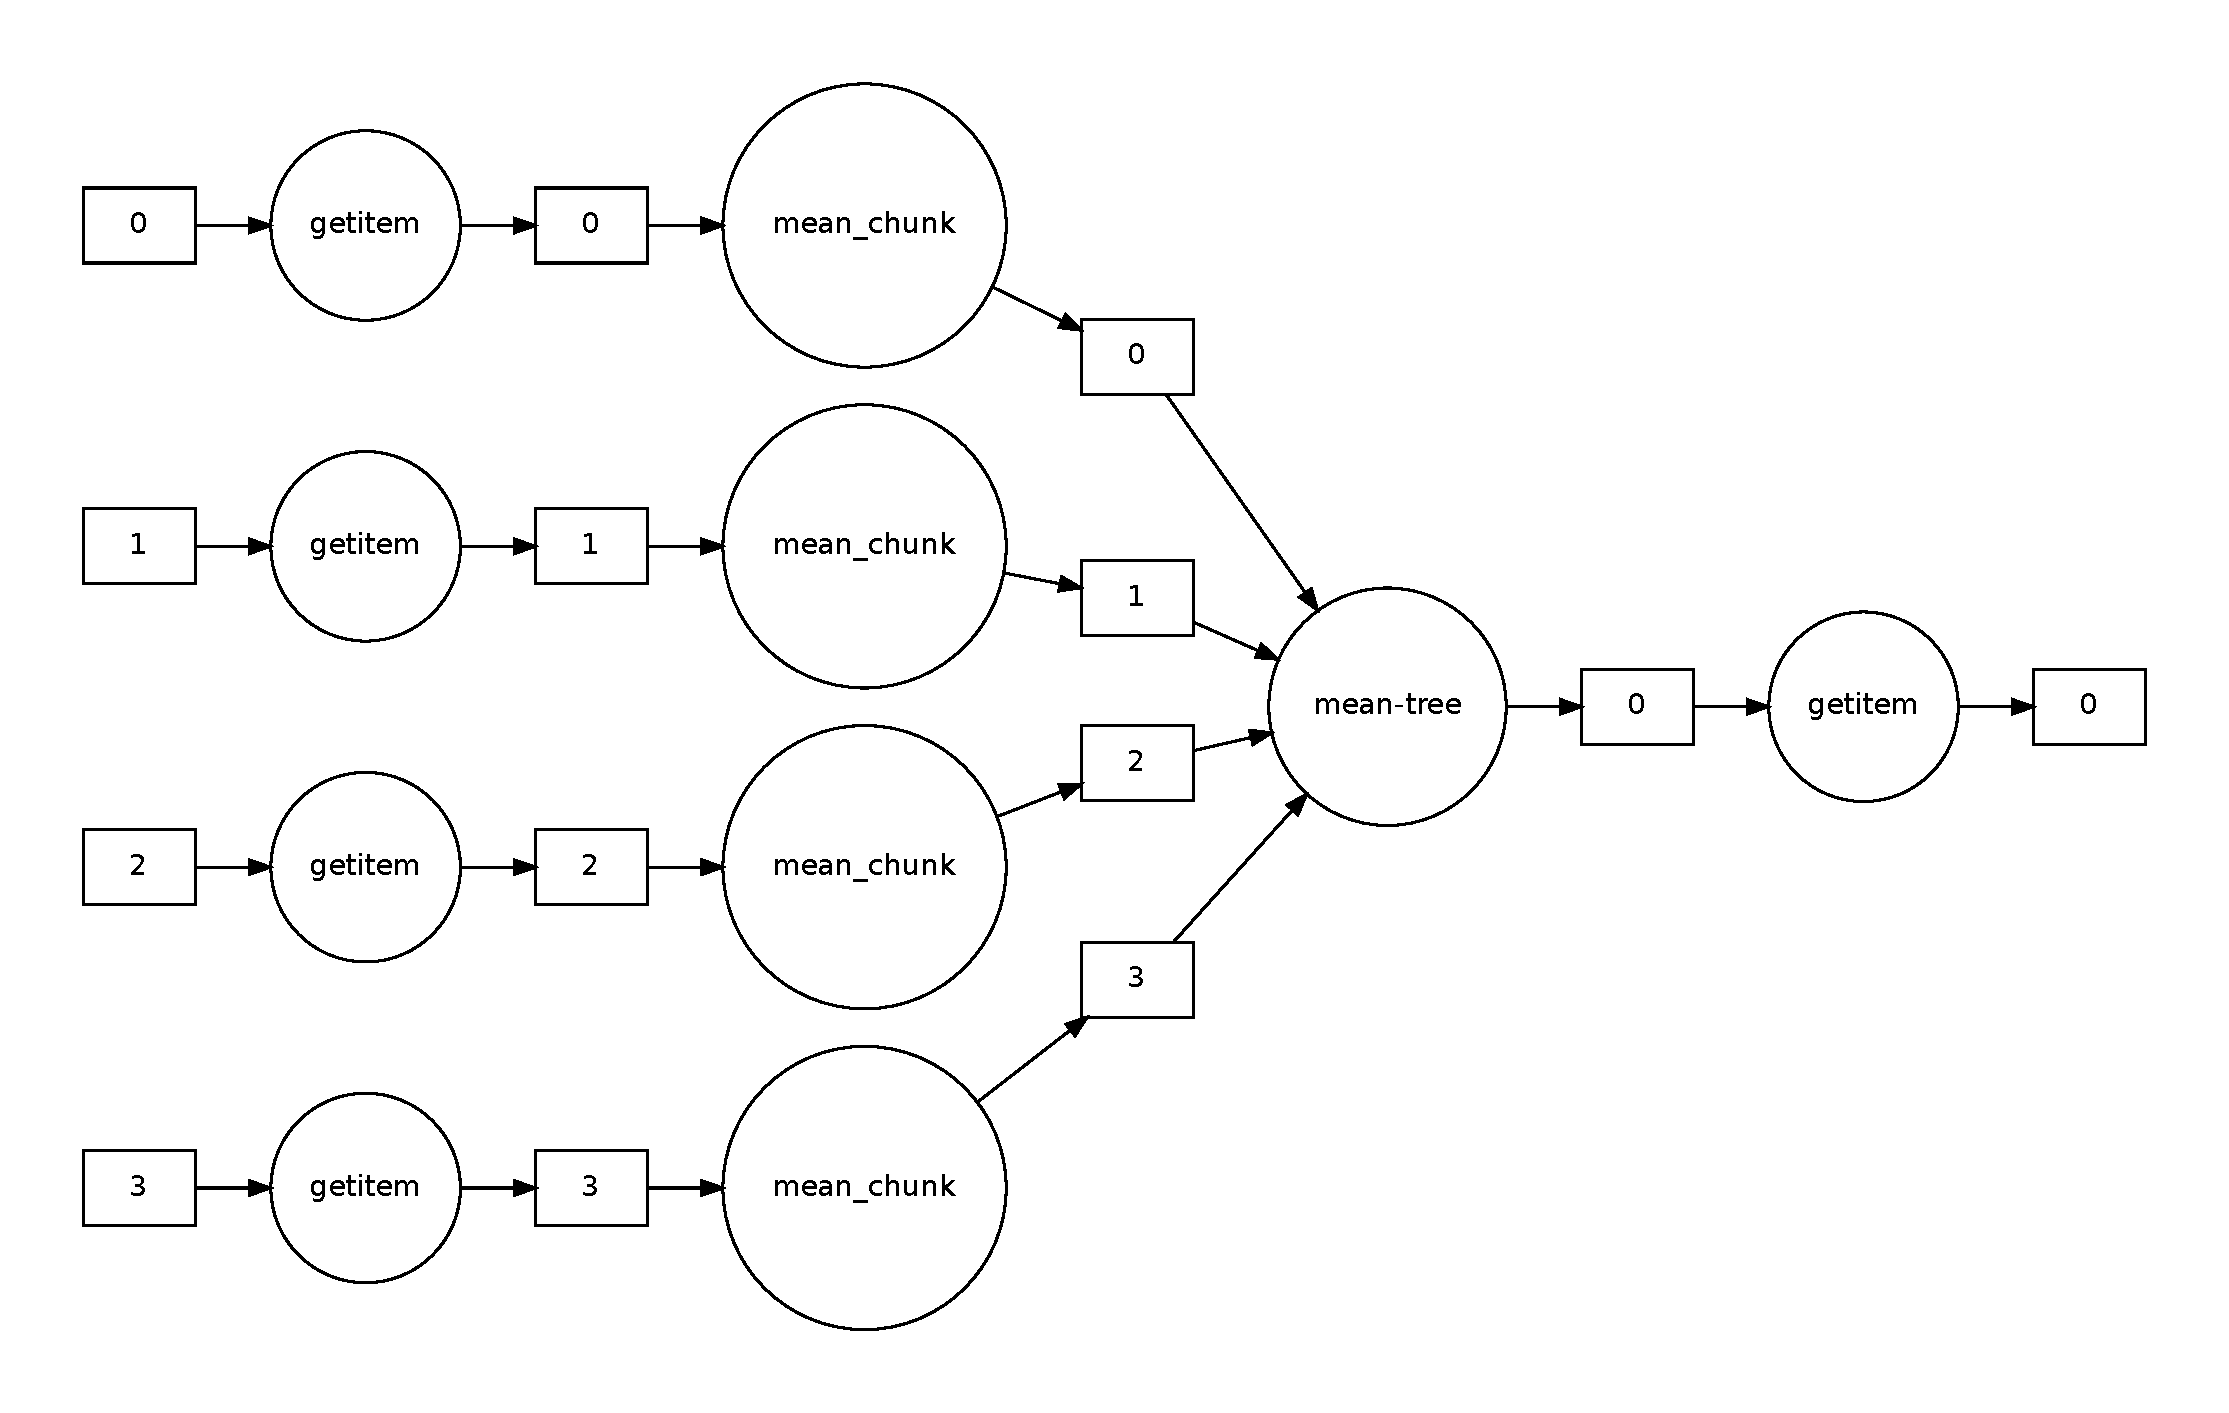
\includegraphics[width=\linewidth]{imgs/dask-dataframe-1-graph}
	\end{minipage}
	\caption{\dask{} DataFrame query and its corresponding task graph}
	\label{lst:dask-dataframe-example-1}
\end{listing}

Specialized types of task graphs are also commonly used to parallelize \emph{dataframe}
processing, which is a popular approach for performing exploratory data analytics and
\gls{olap} queries over two-dimensional tabular datasets (dataframes). Tools such as
\dask{} DataFrame~\cite{dask}, Modin~\cite{modin},
Vaex~\cite{vaex} or CuDF~\cite{cudf} offer Python or
\gls{sql} interfaces for expressing queries over dataframes, and then translate these
queries into task graphs that are executed on parallel machines, distributed clusters or
\gls{gpu} accelerators. Users of these tools do not even necessarily have to know
that they are interacting with task graphs, since their usage is mostly an internal implementation
detail. \Autoref{lst:dask-dataframe-example-1} shows a short Python program that leverages the
\dask{} DataFrame \gls{api} for performing a query on a dataframe
loaded from a \gls{csv} file. The query is internally translated by
\dask{} to the task graph shown on the right side of the figure, which can then be
executed e.g.\ on a distributed cluster.

DataFrame processing is often used in scientific workflows. However, it typically represents only a
certain part of the workflow (e.g.\ a single task or a set of tasks), and it is typically not used
to define the structure of the whole workflow.

While MapReduce, DataFrame processing or other similar models are useful for computations that have
a predictable structure, they are not always general enough to express complex
\gls{hpc} scientific workflows. We will thus further only consider tools and models
that allow executing arbitrary task graphs.

\subsection{Task granularity}
\label{sec:task-granularity}
An important aspect of tasks is their \emph{granularity}, which determines how much work the
task performs and into how many subtasks it could be potentially divided to achieve more
parallelization opportunities. In an extreme case, a \emph{coarse-grained} (low granularity) task could represent
the whole computation that we want to perform, while a \emph{fine-grained} (high granularity) task could represent
merely the execution of a single \gls{cpu} instruction. With an increasing
granularity, each task performs less work, and the whole workflow will thus have to be divided into
a larger number of tasks. This makes it easier to parallelize the workflow; however, it also
increases the overall overhead introduced by the task runtime, which has to manage and schedule
more tasks. The same properties also apply inversely for a decreasing granularity of tasks.

Since tasks represent arbitrary computations, it is not always straightforward to determine how
granular they are. Usually it is much simpler to use a proxy metric for task granularity based on
the duration it takes to execute the task. Therefore, if a task executes very quickly, we will
consider that it is highly granular, while if a task takes a long time to execute, we will consider
that it has low granularity.

Task granularity is important primarily because it determines how efficiently a task graph can be
parallelized and if it even makes sense to distribute it to multiple nodes at all. For example, if
certain tasks would take mere nanoseconds to execute, there would be no point in dynamically load
balancing them across multiple remote nodes, because the overhead of doing so would dwarf the
execution time of the tasks themselves, due to the latency induced by the network communication. In
other words, it would be faster to just execute all such tasks on the local node, rather than
sending them across the network. It could still be worth it to distribute a large number of such
extremely granular tasks to multiple nodes, but the distribution would need to happen in an
amortized way, for example only once at the beginning of the computation, to avoid excessive
communication overhead.

Some task-based programming models focus primarily on high granularity tasks, for example
StarPU~\cite{starpu}, Cilk~\cite{cilk}, HPX~\cite{hpx},
PaRSEC~\cite{parsec}, Legion~\cite{legion}, TBB~\cite{tbb} or
\gls{openmp}~\cite{openmp}\footnote{Note that even though \gls{openmp} has been previously presented as an example of an
explicitly parallel model, it also offers a task system that provides facilities for implicit parallelization.}. In these models, which are
sometimes called \emph{task-parallel}~\cite{task_based_taxonomy}, tasks usually represent either
functions or blocks of code that contain only a few instructions, and are typically relatively
quick to execute (they can run e.g.\ for milliseconds or seconds). While some of these tools also
support distributed computing, their main use-case is to provide intra-node parallelization on
multicore systems with shared memory, and often also to offload computation to attached
accelerators, such as \glspl{gpu} or \glspl{fpga}.

They can be used e.g.\ to implement high-performance numerically intensive computational kernels,
such as matrix multiplication or QR factorization~\cite{qr_factorization}, or to parallelize
recursive algorithms or algorithms with irregular data access patterns. \Autoref{lst:cilk-fibonacci}
shows a program implemented in the Cilk programming language, which calculates the n-th Fibonacci
number using a task-parallel approach.

\begin{listing}
	\begin{minted}[fontsize=\footnotesize, tabsize=4]{c}
cilk int fibonacci(int n)
{
	if (n < 2) {
		return n;
	}
	else
	{
		// Spawn a new task for each recursive call
		int x = spawn fibonaccib(n - 1);
		int y = spawn fibonaccib(n - 2);
		// Wait until the tasks finish with a barrier
		sync;
		return x + y;
	}
}
	\end{minted}
	\caption{Task-parallel Fibonacci calculation using Cilk}
	\centering Source code snippet adapted from~\cite{cilk}.
	\label{lst:cilk-fibonacci}
\end{listing}

Task-parallel models definitely have their place in \gls{hpc}; however, they are not
primarily designed to execute high-level scientific workflows, as they deal with a different set of
challenges and constraints. Therefore, they are not the primary focus of this thesis and will not
be considered in the rest of the text.

There is also a set of task-based tools that reside at the other end of the granularity spectrum,
for example Apache Airflow~\cite{airfow}, Dagster~\cite{dagster},
Prefect~\cite{prefect} or Argo~\cite{argo}. These are commonly labeled as
\emph{Workflow Management Systems}. Although it cannot be said that there is a single distinguishing feature
that would separate these tools from other task runtimes, from my point of view these tools form a
separate category. They are primarily designed for very coarse-grained workflows with a relatively
small number of tasks, they put strong emphasis on workflow reproducibility, data provenance,
execution monitoring (typically through a web interface) and support scheduled execution (i.e.\
``execute this workflow every hour''). They are also typically being applied in cloud environments,
moreso than on supercomputers. This thesis will thus not consider these tools in great detail, as
they are not primarily designed for \gls{hpc} use-cases.

\section*{Summary}
This chapter has introduced various approaches for creating distributed applications designed for
\gls{hpc} clusters. It categorized them into two broad categories, explicitly
parallel and implicitly parallel models, and demonstrated several examples of both approaches.

It has also specified the subset of distributed computing that is most relevant for this thesis. In
particular, this thesis focuses on batch processing task programming models that define
computations using fully general \glspl{dag} and that are designed for distributed
execution on an \gls{hpc} cluster, with tasks whose granularity (duration) typically
spans from (tens of) milliseconds to hours.

These programming models are being commonly used for defining scientific workflows using tools that
will be described in~\Autoref{ch:sota}, which will also discuss various challenges faced by
these tools on \gls{hpc} systems. But before that, the following chapter will first
define a vocabulary of task related terms so that we can refer to them in the rest of the thesis.
